\documentclass[aspectratio=169]{beamer}

\usepackage[utf8]{inputenc}
\usepackage[T1]{fontenc}
\usepackage[french, provide=*]{babel}
\usepackage{tikz}
\usepackage{pgfplots}
\usepackage{listings}
\usepackage{booktabs}
\usepackage{xcolor}

\usetikzlibrary{shapes.geometric, arrows, positioning, calc, matrix}
\pgfplotsset{compat=1.17}

% Theme selection
\usetheme{Madrid}
\usecolortheme{whale}

% Code styling
\definecolor{codegreen}{rgb}{0,0.6,0}
\definecolor{codegray}{rgb}{0.5,0.5,0.5}
\definecolor{codepurple}{rgb}{0.58,0,0.82}
\definecolor{backcolour}{rgb}{0.95,0.95,0.92}

\lstdefinestyle{mystyle}{
    backgroundcolor=\color{backcolour},   
    commentstyle=\color{codegreen},
    keywordstyle=\color{magenta},
    numberstyle=\tiny\color{codegray},
    stringstyle=\color{codepurple},
    basicstyle=\ttfamily\scriptsize,
    breakatwhitespace=false,         
    breaklines=true,                 
    captionpos=b,                    
    keepspaces=true,
    numbers=none,
    showspaces=false,                
    showstringspaces=false,
    showtabs=false,                  
    tabsize=2,
    language=C++
}
\lstset{style=mystyle}

\title{Optimisation du Game of Life sur GPU}
\subtitle{De l'implémentation naïve aux registres 64 bits}
\author{Hugo}
\date{16 Février 2026}

\begin{document}

\begin{frame}
    \titlepage
\end{frame}

\begin{frame}{Introduction}
    \begin{itemize}
        \item \textbf{Objectif :} Accélérer la simulation du Jeu de la Vie de Conway sur GPU (CUDA).
        \item \textbf{Plateforme :} NVIDIA GeForce GTX 1070.
        \item \textbf{Métrique :} Frames Per Second (FPS) sur une grille large.
        \item \textbf{Stratégie :} Réduire les accès mémoire et maximiser le parallélisme.
    \end{itemize}
\end{frame}

\section{Approche Naïve}

\begin{frame}{V1 \& V2 : Approche Naïve (Global Memory)}
    \begin{columns}
        \column{0.5\textwidth}
        \textbf{Principe :}
        \begin{itemize}
            \item 1 thread = 1 cellule.
            \item Lecture directe en mémoire globale pour chaque voisin (8 lectures/thread).
            \item V1 : Calcul booléen.
            \item V2 : Branchements (If/Else).
        \end{itemize}

        \vspace{0.5cm}
        \textbf{Problème :}
        \begin{itemize}
            \item Latence mémoire élevée.
            \item Redondance des lectures (chaque cellule est lue 9 fois par des threads voisins).
        \end{itemize}

        \column{0.5\textwidth}
        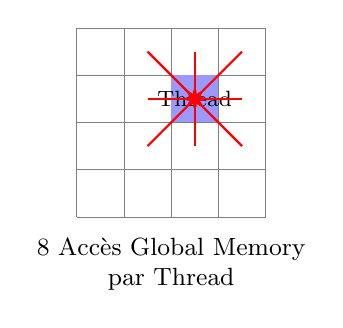
\begin{tikzpicture}[scale=0.6]
            \draw[step=1cm,gray,very thin] (0,0) grid (4,4);
            \fill[blue!40] (2,2) rectangle (3,3); 
            \node[font=\footnotesize] at (2.5,2.5) {Thread};
            
            \foreach \x in {1,2,3} {
                \foreach \y in {1,2,3} {
                    \ifnum\x=2
                        \ifnum\y=2
                        \else
                            \draw[->, red, thick] (\x+0.5,\y+0.5) -- (2.5,2.5);
                        \fi
                    \else
                        \draw[->, red, thick] (\x+0.5,\y+0.5) -- (2.5,2.5);
                    \fi
                }
            }
            \node[align=center, font=\small] at (2,-1) {8 Accès Global Memory\\par Thread};
        \end{tikzpicture}
    \end{columns}

    \vspace{0.5cm}
    \centering
    \alert{Performance : $\approx$ 1000 - 1050 FPS}
\end{frame}

\section{Shared Memory}

\begin{frame}{V3 : Shared Memory \& Tuiling}
    \begin{columns}
        \column{0.5\textwidth}
        \textbf{Optimisation :}
        \begin{itemize}
            \item Chargement collaboratif d'une tuile (Tile) en mémoire partagée (rapide).
            \item Ajout d'un \textbf{Halo} pour gérer les bords.
            \item Accès Globaeuix réduits drastiquement.
        \end{itemize}
        
        \vspace{0.2cm}
        \begin{block}{Gain}
            Réutilisation des données entre threads voisins via le cache L1/Shared.
        \end{block}

        \column{0.5\textwidth}
        \centering
        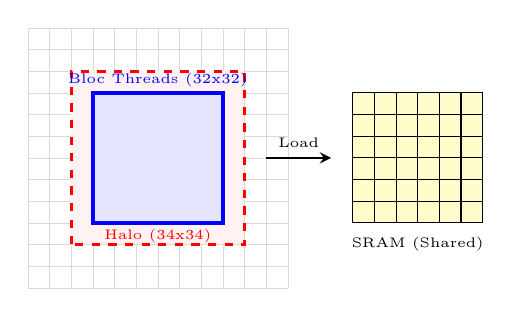
\begin{tikzpicture}[scale=0.55]
            % Grille Globale
            \draw[step=0.5cm,gray!30,very thin] (-1,-1) grid (5,5);
            
            % Halo
            \draw[line width=1pt, red, dashed, fill=red!5] (0,0) rectangle (4,4);
            \node[red, font=\tiny] at (2,0.2) {Halo (34x34)};
            
            % Bloc
            \draw[line width=1.5pt, blue, fill=blue!10] (0.5,0.5) rectangle (3.5,3.5);
            \node[blue, font=\tiny] at (2,3.8) {Bloc Threads (32x32)};
            
            \draw[->, >=stealth, thick] (4.5,2) -- (6,2) node[midway, above, font=\tiny] {Load};
            
            % Shared Memory
            \begin{scope}[shift={(6.5,0.5)}]
                \draw[fill=yellow!20] (0,0) rectangle (3,3);
                \draw[step=0.5cm, black, thin] (0,0) grid (3,3);
                \node[font=\tiny] at (1.5,-0.5) {SRAM (Shared)};
            \end{scope}
        \end{tikzpicture}
    \end{columns}
    \vspace{0.3cm}
    \centering
    \textbf{Performance : 1165 FPS (+10\%)}
\end{frame}

\section{Lookup Table}

\begin{frame}{V4 : Lookup Table (LUT)}
    \begin{columns}
        \column{0.4\textwidth}
        \textbf{Changement de Paradigme :}
        \begin{itemize}
            \item Précalculer toutes les évolutions possibles pour un petit bloc.
            \item Un voisinage $4 \times 4$ (16 bits) détermine l'état futur du centre $2 \times 2$.
            \item \textbf{Vectorisation :} 1 thread calcule 4 pixels d'un coup.
            \item Plus de logique conditionnelle, juste un accès tableau.
        \end{itemize}

        \column{0.6\textwidth}
        \centering
        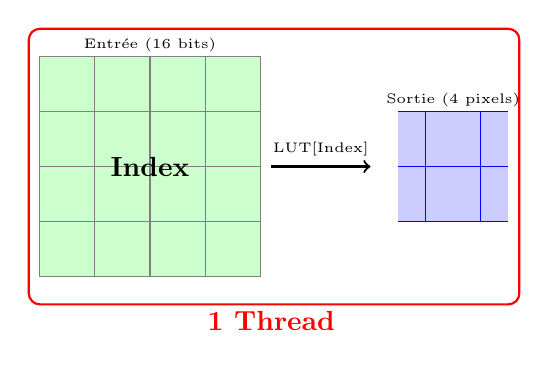
\begin{tikzpicture}[scale=0.7]
            % Grille 4x4 Input
            \fill[green!20] (0,0) rectangle (4,4);
            \draw[step=1cm, gray] (0,0) grid (4,4);
            \node[font=\tiny] at (2,4.2) {Entrée (16 bits)};
            \node[font=\bfseries] at (2,2) {Index};

            % Output 2x2
            \draw[->, thick] (4.2, 2) -- (6, 2) node[midway, above, font=\tiny] {LUT[Index]};
            
            \fill[blue!20] (6.5, 1) rectangle (8.5, 3);
            \draw[step=1cm, blue] (6.5,1) grid (8.5,3);
            \node[font=\tiny] at (7.5, 3.2) {Sortie (4 pixels)};
            
            % Indicateur 1 thread
            \draw[red, thick, rounded corners] (-0.2,-0.5) rectangle (8.7, 4.5);
            \node[red, font=\bfseries] at (4.2, -0.8) {1 Thread};
        \end{tikzpicture}
    \end{columns}
    
    \vspace{0.5cm}
    \centering
    \alert{\Large Performance : 2455 FPS (+110\%)}
\end{frame}

\section{Optimisation Finale}

\begin{frame}{V5 : Bit-Patching \& Registres 64-bits (Le Concept)}
    \begin{columns}
        \column{0.6\textwidth}
        \textbf{Problematique :}
        La V4 est rapide mais fait encore beaucoup d'accès mémoire pour construire l'index 16-bits.
        
        \vspace{0.2cm}
        \textbf{Solution "Bit-Patching" :}
        \begin{enumerate}
            \item Stocker la grille sous forme d'entiers \texttt{uint16\_t} ($4 \times 4$ pixels).
            \item Charger les 9 voisins ($3 \times 3$ blocks) en registres.
            \item Construire un \textbf{"Super-Patch"} virtuel de $6 \times 6$ ou $8 \times 8$ bits dans un seul registre \texttt{uint64\_t}.
            \item Extraire les index LUT par décalages de bits (shift).
            \item \textbf{Zéro accès mémoire} pendant le calcul.
        \end{enumerate}

        \column{0.4\textwidth}
        \centering
        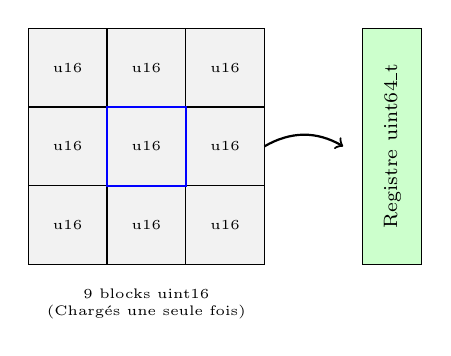
\begin{tikzpicture}[scale=0.5]
            % 3x3 Blocks
            \foreach \x in {0,1,2} {
                \foreach \y in {0,1,2} {
                    \draw[fill=gray!10] (\x*2, \y*2) rectangle (\x*2+2, \y*2+2);
                    \node[font=\tiny] at (\x*2+1, \y*2+1) {u16};
                }
            }
            \draw[blue, thick] (2,2) rectangle (4,4); % Center
            
            % Arrow to Register
            \draw[->, thick, bend left] (6, 3) to (8, 3);
            
            % Register
            \draw[fill=green!20] (8.5, 0) rectangle (10, 6);
            \node[rotate=90, font=\scriptsize] at (9.25, 3) {Registre uint64\_t};
            
            \node[align=center, font=\tiny] at (3,-1) {9 blocks uint16\\(Chargés une seule fois)};
        \end{tikzpicture}
    \end{columns}
\end{frame}

\begin{frame}[fragile]{V5 : Détail du Bit-Patching (Code CUDA)}
    \textbf{Construction du voisinage sans accès mémoire :}
    \begin{center}
    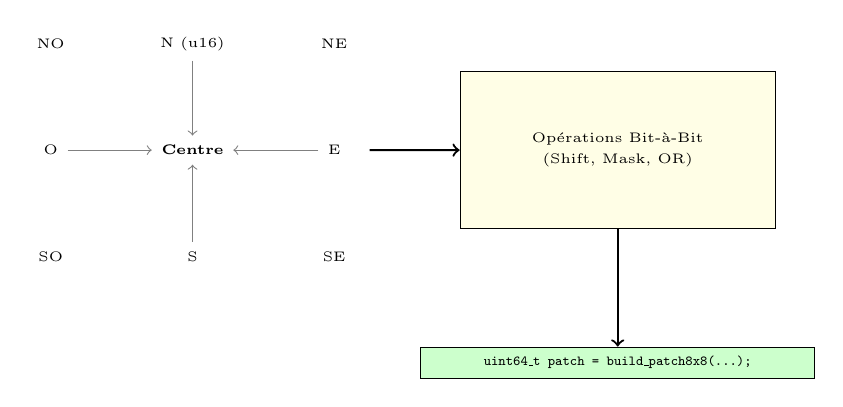
\begin{tikzpicture}[scale=0.9, every node/.style={font=\tiny}]
        % Voisinage abstrait
        \node (N) at (2,3) {N (u16)};
        \node (NO) at (0,3) {NO}; \node (NE) at (4,3) {NE};
        \node (C) at (2,1.5) {\textbf{Centre}};
        \node (O) at (0,1.5) {O}; \node (E) at (4,1.5) {E};
        \node (S) at (2,0) {S};
        \node (SO) at (0,0) {SO}; \node (SE) at (4,0) {SE};
        
        % Data flow
        \draw[->, gray] (N) -- (C); \draw[->, gray] (S) -- (C);
        \draw[->, gray] (O) -- (C); \draw[->, gray] (E) -- (C);
        
        % Bit Operations Box
        \node[draw, fill=yellow!10, minimum width=4cm, minimum height=2cm] (OP) at (8, 1.5) {
            \shortstack{Opérations Bit-à-Bit\\(Shift, Mask, OR)}
        };
        
        \draw[->, thick] (4.5, 1.5) -- (OP);
        
        % Result Register
        \node[draw, fill=green!20, minimum width=5cm] (REG) at (8, -1.5) {
            \texttt{uint64\_t patch = build\_patch8x8(...);}
        };
        \draw[->, thick] (OP) -- (REG);
        
    \end{tikzpicture}
    \end{center}
    
    \vspace{-0.5cm}
    % Code listing (moved out of columns to avoid fragile/column interaction)
\begin{lstlisting}
// Extrait de conway.cu
uint64_t patch = 0;
// Reconstitution ligne par ligne (bits)
// Exemple pour la partie Nord (Row 0 patch)
uint8_t mid = (N >> (4*src)) & 0xF;
uint8_t left = (NO >> (4*src+2)) & 3; 
// ...
patch |= (uint64_t)row << (8*i);
\end{lstlisting}
\begin{itemize}
    \item Tout se passe dans les registres.
    \item Haute intensité arithmétique.
    \item Parallélisme de donnée maximal.
\end{itemize}
\end{frame}

\section{Résultats}

\begin{frame}{Synthèse des Performances}
    \centering
    % Simplified results table (pgfplots chart temporarily disabled to avoid compilation issue)
    \vspace{0.5cm}
    \begin{tabular}{l r}
        \toprule
        Version & FPS \\
        \midrule
        V1 (Naïve Bool) & 1001.00 \\
        V2 (Naïve If) & 1057.26 \\
        V3 (Shared) & 1165.18 \\
        V4 (LUT 4x4) & 2455.34 \\
        V5 (LUT u16+Reg) & 3208.89 \\
        \bottomrule
    \end{tabular}
\end{frame}

\begin{frame}{Conclusion}
    \begin{block}{Résumé des gains}
        \begin{itemize}
            \item \textbf{Global $\rightarrow$ Shared Ops :} Gain modéré (+10\%).
            \item \textbf{Logique $\rightarrow$ LUT :} Gain massif par vectorisation (x2.1).
            \item \textbf{Shared $\rightarrow$ Registres (Bit-Patching) :} Gain final (+30\%).
        \end{itemize}
    \end{block}

    \vspace{0.5cm}
    \textbf{Performance finale :}
    \begin{itemize}
        \item \textbf{x3.2} plus rapide que l'implémentation naïve.
        \item Utilisation optimale de la bande passante et des registres 64 bits du GPU.
    \end{itemize}
\end{frame}

\end{document}
